\documentclass[spanish]{article}
\usepackage[spanish]{babel}
\usepackage{amsmath}
\usepackage{amssymb}
\usepackage[utf8]{inputenc}
\usepackage{vmargin}
\usepackage{graphicx}
\usepackage{wrapfig}
\usepackage[export]{adjustbox}


\begin{document}

\includegraphics[width=1\textwidth, right]{./imagenes/logos.png}
	\setpapersize{USletter}
	\setmarginsrb{30mm}{30mm}{30mm}{30mm}{0pt}{0mm}{0pt}{0mm}
	
	\begin{center}
	{\Large Análisis de Algoritmos, Sem: 2018-1, 3CV2 Práctica 9, 23 de Noviembre del 2017}\\
{\huge {\bf Práctica 10: Verificación en Tiempo Polinomial}} \\
{\large {\bf Salgado Alarcon Genaro, Padilla Calderon Jose Manuel}\\
Escuela Superior de Cómputo \\
Instituto Politécnico Nacional}\\
isomaelking@gmail.com, genaro\_yen13@hotmail.com\\
	\end{center}

	
	\bigskip
	
	\bigskip
	
	\bigskip
	
	{\LARGE {\bf Primero}}\\
	
	En este trabajo vamos a ver la implementación de la solución de un problema NP, la cuál, será aquel de ciclos Hamiltonianos. Este problema se va tratar analizando su tiempo de ejecución, donde dicho tiempo debe de ser polinomial. Además, se dará uso de gráficas y artificios matemáticos para comprobar que dicho tiempo antes mencionado.

	\bigskip


	{\Large {\bf Palabras Clave}}\\
	\begin{itemize}
		\item Algoritmo
		\item Hamiltoniano
		\item NP
		\item Grafo
		\item Ciclo
	\end{itemize}
	
	\section{Introducci\'on}
	El algoritmo que verifica ciclos Hamiltonianos en un grafo, consiste en que...la verdad, no tengo mucha idea que escribir aquí. Lo que escribo es realmente conceptos de más abajo...
\newpage
	\section{Conceptos B\'asicos}
	Para la correcta comprension de este trabajo, es necesario definir algunos terminos tales como $\theta$, O y $\Omega$.\\
	 $\theta$(n):\\
		Sea g(n) una función. Se define  $\theta$ (g(n)) como:\\
		
		 	$\theta$(g(n)) = $\{ f(n) \quad | \quad \exists c1,c2>0 \quad \& \quad n_{0}>0 \quad \mid \quad \forall n>=n_{0} \quad 0<= c1g(n) <= f(n) <= c2g(n) \}$
	\bigskip		 	
		 	
	O(n):\\
		Sea  g(n)  una función, O(n) (el pero de los casos) se define como:\\
		
			\hspace{1cm}O(n)=$\{f(n) \quad | \quad \exists c >0 \quad \& \quad n_{0}>0 \quad | \quad f(n) <= Cg(n) \quad \forall  n>= n_{0} \}$
	\bigskip
	
	$\Omega$(n):\\
	Sea  g(n)  una función. Se define $\Omega$ (g(n)) (el mejor de los casos) como:\\

		\hspace{1cm}$\Omega$(g(n)) =$\{f(n) \quad | \quad \exists c >0 \quad \& \quad n_{0}>0 \quad \mid \quad  0<= cg(n)<= f(n) \quad \forall n>= n_{0} \}$
	\bigskip
	
	El algoritmo de encontrar un ciclo Hamiltoniano consiste en cruzar todos los vértices de un grafo sin pasar una segunda vez por alguno de ellos. No obstante, es necesaria otra condición para que dicho camino encontrado sea un ciclo hamiltoniano:

	\begin{center}
		\textit{Un ciclo hamiltoniano es aquella trayectoria donde cruza por todos los vértices del grafo analizado, pero el final de dicho trayecto de terminar en el vértido donde se comenzó. En caso contrario, esta trauectoria se conocerá como Camino Hamiltoniano}
	\end{center}

	A continuación, en la figura 1 se muestra de manera gráfica dicha condición. Podemos tener en un grafo caminos hamiltonianos pero no necesariamente que también sean ciclos hamiltonianos.

	\begin{center}
		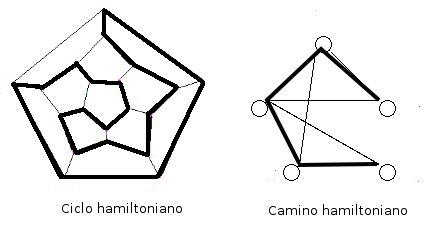
\includegraphics[width=0.55\textwidth]{./imagenes/figura1.png}\\
		Figura 1. Camino Hamiltoniano vs Ciclo Hamiltoniano\\
	\end{center}

	De manera formal, un ciclo Hamiltoniano es necesario que se encuentre en un grafo Hamiltoniano. Éste se puede describir de la siguiente forma:\\
	
	Sea G un grafo conexo. Si existe W $\subset$  V tal que G / W tiene $c$ componentes conexas con c $>$ $|W|$, entonces G no es Hamiltoniano\\

	Para resolver este problema es posible de diferentes maneras. La más rápida de visualizar es por medio de la fuerza bruta, es decir, probar cada combinación entre los vértices del grafo, pero esta solución se vuelve muy lenta; supongamos que tenemos un grafo de n vértices, si se desea realizar todas las combinaciones posibles, tendríamos un total de n!. Como vemos, incrementa factorialmente el tiempo de ejecución por medio de la fuerza bruta. \\	
	
	\newpage	

	Por este motivo, dicho problema se encuentra en la categoría de NP; aunque el incremento de vértices sea pequeño, el tiempo de ejecución crecerá enormemente. Es cierto que hay otros algoritmos que reducen  dicho tiempo, como es el caso del algoritmo de Bellman, Held y Karp, donde usan programación dinámica y el tiempo es de O($n^2$$2n$). Aún con algoritmos con menor tiempo, éstos siguen siendo de carácter exponensial, que para nuestros propósitos sigue teniendo una tasa de crecimiento alta.

	\section{Experimentaci\'on y Resultados}
		
	\subsection{Implemente el algortimo de Verificación de Hamilton que verifique en tiempo polinomial que el certificado C  es o no un ciclo Hamiltoniano del grafo G}

	{\large{ {\bf i) Mediante gráficas, muestre que el certificado es o no un ciclo Hamiltoniano en tiempo polinomial.}}}\\

	{\large{ {\bf i) Analíticamente, muestre que el certificado es o no un ciclo Hamiltoniano en tiempo polinomial.}}}\\
	
	\section{Conclusi\'on General}

	\bigskip

	***

	\bigskip

	\newpage

	\section{Conclusiones Individuales}

	\bigskip

	{\large{\bf Salgado Alarcon Genaro}}\\

	\bigskip

	***

	\bigskip

	{\large{\bf Padilla Calderon Jose Manuel}}\\
	
	\bigskip

	***

	\bigskip


	\section{Bibliografía}
	\begin{itemize}
		\item Brassard, G. (1997). Fundamentos de Algoritmia. España: Ed. Prentice Hall. ISBN 		848966000X
		\item Harel, D. (2004). Algorithmics: The spirit of Computing (3rd. Ed). Estados Unidos de América: Addison
Wesley. ISBN-13: 978-0321117847
	\end{itemize}


\end{document}